For the curious reader, we wanted to include here an illustration and a description of the three components of the demonstration we presented above in Section~\ref{sec:4:gnuradio}.

The code corresponding to the following components is written in \texttt{C++} and \texttt{Python} for the hand-written blocks, and using the GUI of the GNU Radio Companion software.
The flow-graphs are saved as XML files, and the complete code of our demo is fully available online, open-sourced under GPLv3 license, at
\href{https://bitbucket.org/scee_ietr/malin-multi-arm-bandit-learning-for-iot-networks-with-grc}{\texttt{bitbucket.org/scee\_ietr/malin-multi-arm-bandit}\\\texttt{-learning-for-iot-networks-with-grc/}}.

\subsubsection*{Random traffic generator}

Figure~\ref{fig:4app:USRP_TX_PU__v1__simple_grc} shows the \textbf{random traffic generator} flow-graph.
\texttt{Generator} is the only hand-written block, which is configured with a list of active channels, a list of occupancy rate, and constants about the PHY layer (preamble length and data length).
It uses one USRP equipped with one antenna, as it only emits data (by using the ``UHD: USRP'' block in``Sink'' mode).

\begin{figure}[!h]
	% \centering
    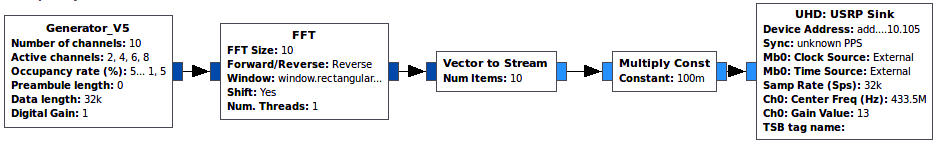
\includegraphics[width=1.02\textwidth]{2-Chapters/4-Chapter/Images/USRP_TX_PU__v1__simple_grc.png}
    \caption{The \textbf{random traffic generator} flow-graph.}
    \label{fig:4app:USRP_TX_PU__v1__simple_grc}
\end{figure}


\subsubsection*{IoT base station}

The \textbf{IoT base station} is presented in Figure~\ref{fig:4app:USRP_RX_BTS__v1__simple_grc} below.
%
We wrote the following blocks:
\begin{itemize}
    \item
    1) the \texttt{Demodulator} block, which is configured with a list of detection threshold (on the received power),
    \item
    2) the \texttt{Check\_ack} block, which is configured with a maximum block error and an accepted error rates (to decide when a message is close enough to an acknowledgement),
    \item
    and finally
    3) the \texttt{send\_ack} block, which is configured with the list of active channels, and knowledge about the PHY layer (delay before sending the Ack and its length).
\end{itemize}
All blocks need to know the constants about the PHY layer (preamble length and data length).
The base station uses one USRP board equipped with two antennas,
to emit and receive data (by using ``Sink'' and ``Source'' modes).

\begin{figure}[!h]
	% \centering
    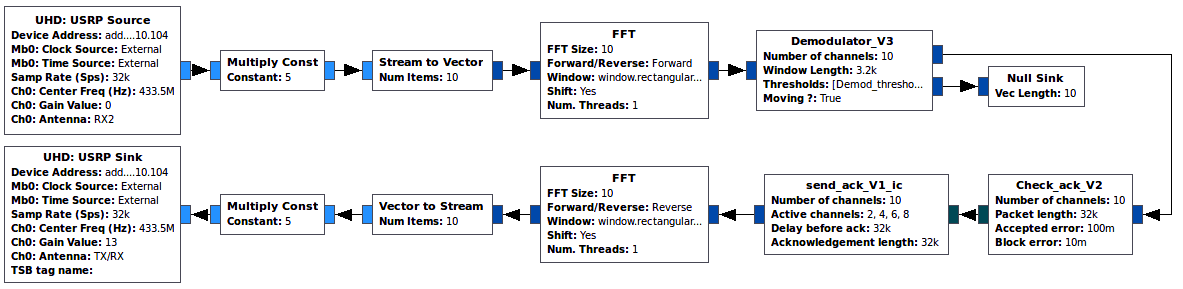
\includegraphics[width=1.00\textwidth]{2-Chapters/4-Chapter/Images/USRP_RX_BTS__v1__simple_grc.png}
    \caption{The \textbf{IoT base station} flow-graph.}
    \label{fig:4app:USRP_RX_BTS__v1__simple_grc}
\end{figure}


\subsubsection*{IoT dynamic device}

Figure~\ref{fig:4app:USRP_TX_SU__v1__simple_grc} below shows the \textbf{IoT dynamic device} flow-graph.
The hand-written blocks are
\begin{itemize}
    \item
    1) the \texttt{Renormalized\_ack} block, which is configured with the list of active channels and extra knowledge about the PHY layer (preamble length, message length, and a threshold to tune detection of the incoming Ack),
    \item
    2) the \texttt{Demodulator} and 3) the \texttt{Check\_ack} blocks, both shared with the IoT gateway,
    \item
    and finally 4) the \texttt{generator\_SU} block, which embeds the \UCB{} or Thompson Sampling algorithm, and which is configured with the list of active channels.
\end{itemize}
Most blocks need to know constants about the PHY layer (preamble length and data length).
Any of the IoT dynamic devices also uses one USRP board equipped with two antennas,
to emit and receive data (``Sink'' and ``Source'' modes).

We note the difference between the base station and the end-devices.
The base station uses its Rx antenna to scan the entire range of the $K$ channels, at all time steps ; while dynamic devices use their Rx antennas only to listen for the acknowledgement sent by the base station if it received and decoded its uplink packet.
After each transmission, the dynamic device listens to one channel during a certain time interval, in the channel used for uplink transmission.

\begin{figure}[!h]
	% \centering
    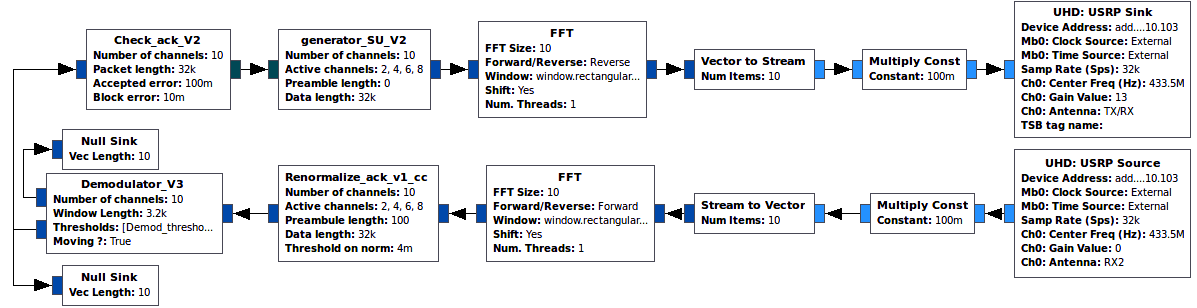
\includegraphics[width=1.00\textwidth]{2-Chapters/4-Chapter/Images/USRP_TX_SU__v1__simple_grc.png}
    \caption{The \textbf{IoT dynamic device} flow-graph.}
    \label{fig:4app:USRP_TX_SU__v1__simple_grc}
\end{figure}
